\documentclass[AtomicOptical1Notes.tex]{subfiles}

\begin{document}

\begin{center}\huge Week 1: Classical Resonances\end{center}

\section{Resonances - an overview}

	\subsection{Introduction to resonance}
				\begin{itemize}
					\item Resonance - any periodic variation of some variable. When you drive a system with a variable frequency, you observe a peak at resonant frequency.
					\item Atomic Physics is interested with every single possible aspect of resonance. Resonance is the language physicists talk to atoms with.
					\item Oscillators are characterized by the sharpness of the resonance (Q - quality factor) which is a ratio of the frequency width of the resonance and its resonant frequency. Q is the number of oscillations that can be observed before the oscillation decays away.
					\item In Atomic Physics oscillators are characterized by extremely high Q factors
						\begin{itemize}
							\item optical oscillators: $10^{15}$ Hz (light frequency) $\Rightarrow$ $Q = 10^6$	(with doppler broadening), $Q = 10^{15}$ (without doppler broadening, eg. atom in optical lattice in metastable levels)
							\item mechanical oscillators: eg. quartz $Q = 10^4$ - $10^6$
							\item micromechanical oscillators: $Q = 10^5$ (eg. whispering gallery mode can have $Q = 10^9$, where light circulates around the circle of the mushroom-like structure)
							
							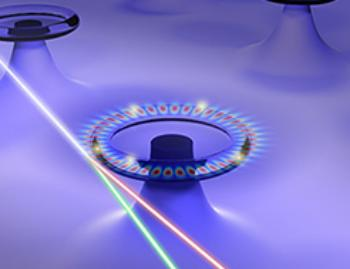
\includegraphics{whispering}
							
							\item astronomical oscillators: earth rotation: $Q = 10^7$, neutron star: $Q = 10^{10}$
						\end{itemize}
					\item "Useful" resonances are reproducible and connected by theory to fundamental constants.
					\item Rydberg constant ($R = 1.097... * 10^7 m^{-1}$) is the most accurately known constant in physics because it can be directly measured by performing spectroscopy experiments with hydrogen. Measuring fundamental constants more accurately is very important in understanding the world.
					\item Typical resonance lineshape is lorentzian which is proportional to Im$\left(\frac{1}{\omega_0-\omega+i*\frac{\gamma}{2}}\right)$. For lorentzian: $\gamma = $FWHM and $Q = \frac{\omega_0}{\gamma}$.
				\end{itemize}
				
	\subsection{Angular frequency units}
		\begin{itemize}
			\item All parameters should be measured in angular frequency units which are technically $\frac{rad}{s}$, sometimes we use $s^{-1}$. Frequencies (not angular) are measured in Hz.
			\item Good manner is to write angular frequency as $\omega_0 = 2\pi*1\text{MHz} = 6.28 * 10^6 s^{-1}$, \emph{NEVER} $6.28 * 10^{6}$ Hz.
			\item Units for $\gamma$ (temporal decay rate, inverse of dumping time) are $s^{-1}$ (\emph{NOT} Hz).
		\end{itemize}
		
\section{Resonance widths and uncertainty relations}
	\subsection{How precisely can you measure frequencies?}
		\begin{itemize}
			\item Some of the most accurate experiments in physics are done by measuring frequency.
			\item For oscillator oscillating for time $\Delta t$ with finite width of frequency spectrum $\Delta\omega$: $\Delta\omega\Delta t \geq \frac{1}{2}$
		\end{itemize}
	\subsection{Heisenberg limits on quantum and classical systems}
		\begin{itemize}
			\item Heisenberg uncertainty relation is about single measurement on a single quantum system. To increase accuracy of the measurement it can be repeated many times or can be done on a system with many photons.
			\item Using nonlinear process it can be achieved for a single quantum system and a single photon utilizing many energy levels at the same time and jumping many levels at the same time. Precision of such an experiment is better by $\frac{1}{n}$ times, where $n$ is the number of energy levels.
		\end{itemize}
	\subsection{Frequency measurement example: atomic clocks}
		\begin{itemize}
			\item Cesium atom fountain clock, $\omega=2\pi*10$GHz, interrogation time $\Delta t=1$s has fractional linewidth $\frac{\Delta\omega}{\omega}=10^{-11}$. Accuracy of the best cesium fountains is now $10^{-16}$.
			\item Strontium optical clock - extremely narrow transition. Accuracy $6*10^{-18}$!
		\end{itemize}
		
\section{Harmonic oscillators and two-level systems}
	\subsection{Harmonic oscillators vs. two-level systems}
		\begin{itemize}
			\item Two-level system is a system with 2 levels. Harmonic oscillator is a system with infinite number of equidistant levels. 
			\item When some energy is put into the second state of HO, some small energy also goes into every higher level. In two-level system there are no higher levels than second one, so nothing can go higher.
			\item Quantum system can be described as a harmonic oscillator for weak excitation (when there is small energy in excited state).
			\item Two-level system can be saturated (harmonic oscillator can never be saturated). When the second energy level is full adding more energy can't go higher. If a two-level system is not saturated, it behaves like a harmonic oscillator so it behaves completely classical.
		\end{itemize}
	\subsection{Rotating systems vs. 2-level systems}
		\begin{itemize}
			\item Precessing gyroscope has a bound on amplitude. Motion of classical magnetic moments provides a model which captures almost all features of the quantum mechanical two-level system (except for projection, quantum measurement).
		\end{itemize}
\section{Classical magnetic moment in a uniform field}
	\subsection{Magnetic resonance}
		\begin{itemize}
			\item Gyromagnetic ratio ($\gamma$) is a ratio between magnetic moment and angular momentum ($\gv{\mu}=\gamma\v{L}$). From that we can find that derivative of angular momentum is given by: $\dot{\v{L}}=\gamma\v{L}\times\v{B}$. Solution of that equation is a pure precession of $\v{L}$ around $\v{B}$. Precession around the $\v{B}$ is happening at the constant tipping angle with an angular frequency called Larmor frequency $\Omega_L=-\gamma B$.
			
			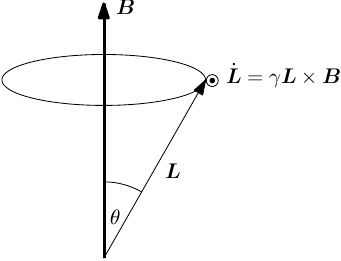
\includegraphics{precession}
			
			\item For an electron $\gamma_e=2\pi*2.8$MHz/G. For classical charge distribution (of particles with the same charge to mass ratio as electrons) gyromagnetic ratio is a half of that: $\gamma=2\pi*\mu_B$ (where $\mu_B = 1.4$MHz/G and is called Bohr magneton).
			\item Proton is heavier than the electron ($\frac{m_p}{m_e}=1836.153$) and therefore $\gamma_P=2\pi*4.2$kHz/G.
		\end{itemize}
		
\end{document}